\section{\acl{soh} and \acl{rul}} \label{sec:soh_rul}

The development of machine learning models for battery prognosis requires clearly defined target variables, namely \acf{soh} and \acf{rul} These metrics serve as key performance indicators to quantify the degradation state of a battery. The following section outlines the methodology used to calculate these ground-truth labels from the experimental cycling data.

The \acf{soh} of a battery provides a snapshot of its current condition relative to its initial, "healthy" state. It is typically expressed as a percentage of the nominal capacity. For the purpose of this study, the \ac{soh} for the nth cycle, denoted as $SoH_n$, is calculated as the ratio of the maximum discharge capacity observed during that cycle to the rated cell capacity, as shown in Equation \ref{eq:soh}.

\begin{equation}
    \mathrm{SoH}_n = \frac{Q_n}{Q_{\text{rated}}}
    \label{eq:soh}
\end{equation}

where $Q_n$ is the maximum discharge capacity recorded for the $n^{th}$ cycle, and $Q_{rated}$ is the rated capacity of a new cell.

A critical limitation in determining the ground-truth \ac{soh} in real-world applications is that batteries rarely undergo a full charge or discharge cycle. This makes it challenging to accurately measure the true capacity at any given time. The controlled laboratory setting used to generate this dataset, where full cycles are performed, provides a consistent and reliable method for calculating this critical ground truth.

The \ac{rul} of a battery represents the number of cycles it can endure before reaching its \ac{eol} condition. The \ac{eol} is a predefined failure threshold, commonly set when the battery's capacity drops to 80\% of its initial rated capacity. The \ac{eol} cycle is therefore defined as the cycle number at which the \ac{soh} first falls to 80\% or below.

\begin{equation}
    \mathrm{EoL} = \min \left\{ n \;\middle|\; \mathrm{SoH}_n \leq 0.80 \right\}
    \label{eq:eol}
\end{equation}

The \ac{rul} for any given cycle n, denoted as $\mathrm{RUL}_n$, is then calculated by subtracting the current cycle number from the \ac{eol} cycle number, as expressed in \cref{eq:rul} below.

\begin{equation}
    \mathrm{RUL}_n = \mathrm{EoL} - n
    \label{eq:rul}
\end{equation}

A significant challenge associated with using cycle count to define \ac{rul} is its limited applicability to real-world scenarios. In our dataset, cycles are a consistent, predictable, and well defined quantity; realistic use-cases often involve irregular charging and discharging patterns, which makes ``cycles'' an unreliable metric. Furthermore, determining the ground truth \ac{rul} for a particular cycle requires having the full degradation data up to the battery's \ac{eol}, which is a common limitation when training \ac{rul} prediction models from incomplete datasets.

Figure \ref{fig:targets_distribution} shows the distribution of both \ac{soh} and \ac{rul} on the Severson dataset \cite{sev2019}. Notably, neither target exhibits a symmetric distribution. The skewed nature  of require a machine learning model that is robust to non-normal data distributions and can effectively capture the non-linear degradation behavior of batteries.


\begin{figure}[H]
    \centering
    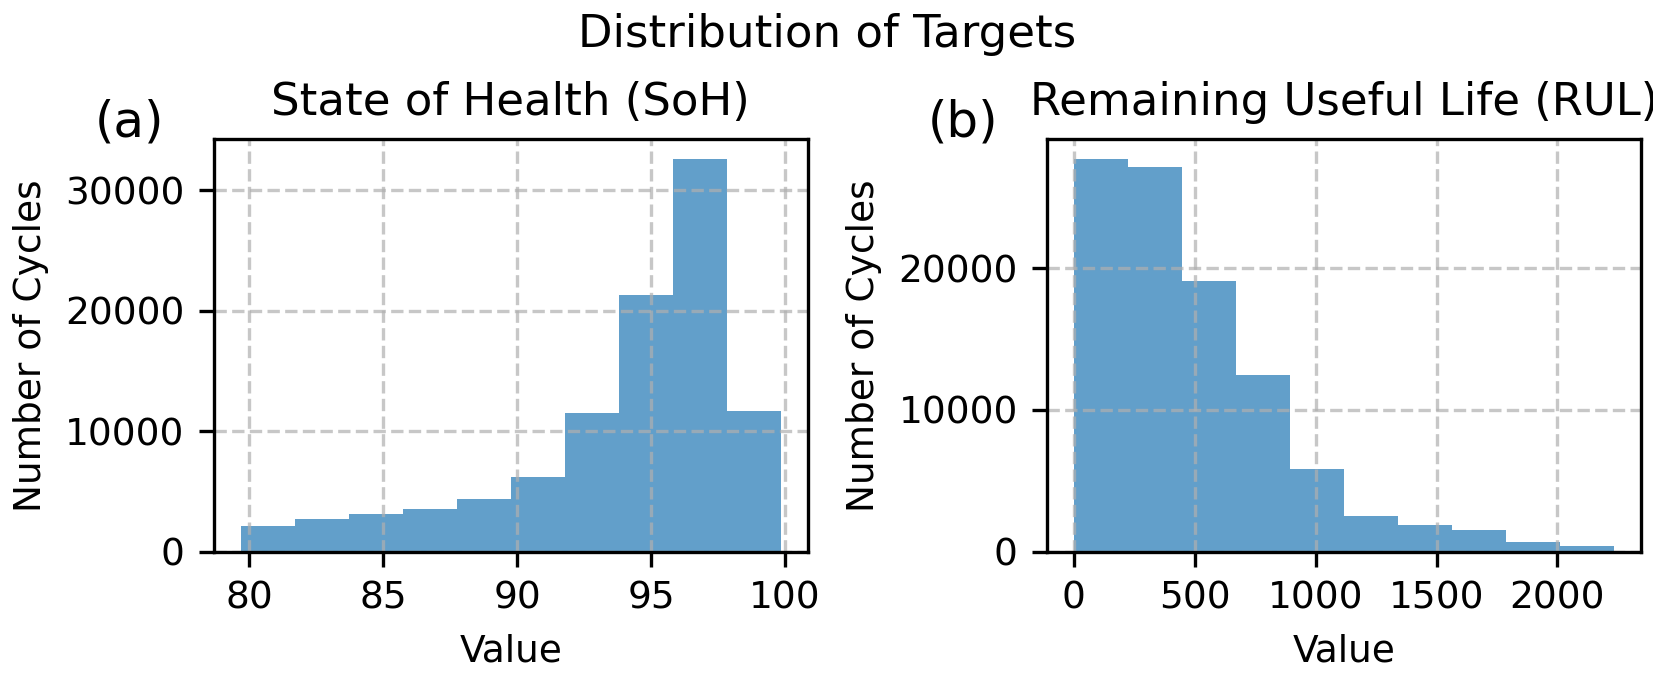
\includegraphics[width=0.8\textwidth]{_img_targets_distribution.png}
    \caption{Distributions of the target variables: (a) \acf{soh} and (b) \acf{rul}, showing the number of cycles across different values.}
    \label{fig:targets_distribution}
\end{figure}
